\documentclass[a4paper,12pt,oneside]{book}

%-------------------------------Start of the Preable------------------------------------------------
\usepackage[english]{babel}
\usepackage{blindtext}
%packagr for hyperlinks
\usepackage{hyperref}
\hypersetup{
    colorlinks=true,
    linkcolor=blue,
    filecolor=magenta,      
    urlcolor=cyan,
}

\urlstyle{same}
%use of package fancy header
\usepackage{fancyhdr}
\setlength\headheight{26pt}
\fancyhf{}
%\rhead{
\includegraphics[width=1cm]{logo}}
\lhead{\rightmark}
\rhead{
\includegraphics[width=1cm]{logo}}
\fancyfoot[RE, RO]{\thepage}
\fancyfoot[CE, CO]{\href{http://www.e-yantra.org}{www.e-yantra.org}}

\pagestyle{fancy}

%use of package for section title formatting
\usepackage{titlesec}
\titleformat{\chapter}
  {\Large\bfseries} % format
  {}                % label
  {0pt}             % sep
  {\huge}           % before-code
 
%use of package tcolorbox for colorful textbox
\usepackage[most]{tcolorbox}
\tcbset{colback=cyan!5!white,colframe=cyan!75!black,halign title = flush center}

\newtcolorbox{mybox}[1]{colback=cyan!5!white,
colframe=cyan!75!black,fonttitle=\bfseries,
title=\textbf{\Large{#1}}}

%use of package marginnote for notes in margin
\usepackage{marginnote}

%use of packgage watermark for pages
%\usepackage{draftwatermark}
%\SetWatermarkText{
\includegraphics{logo}}
\usepackage[scale=2,opacity=0.1,angle=0]{background}
\backgroundsetup{
contents={
\includegraphics{logo}}
}

%use of newcommand for keywords color
\usepackage{xcolor}
\newcommand{\keyword}[1]{\textcolor{red}{\textbf{#1}}}

%package for inserting pictures
\usepackage{graphicx}

%package for highlighting
\usepackage{color,soul}

%new command for table
\newcommand{\head}[1]{\textnormal{\textbf{#1}}}


%----------------------End of the Preamble---------------------------------------


\begin{document}

%---------------------Title Page------------------------------------------------
\begin{titlepage}
\raggedright
{\Large eYSIP2018\\[1cm]}
{\Huge\scshape CNC Growbox \\[.1in]}
\vfill
\begin{flushright}
{\large Intern 1 Devang Joshi \\}
{\large Intern 2 Ujwal Pawar \\}
{\large Intern 3 Harsh Lunia \\}
{\large Lohit Penubaku, Kedar Anavardekar, Ajit Harpude \\}
{\large Duration of Internship: $ 21/05/2018-06/07/2018 $ \\}
\end{flushright}

{\itshape 2018, e-Yantra Publication}
\end{titlepage}
%-------------------------------------------------------------------------------

\chapter[Project Tag]{CNC for Growbox}
\section*{Abstract}
The present revolution in agriculture(Agri 4.0), demands food for next generations. As a step towards contributing to the revolution we had a GrowBox designed, which enabled us to grow selected veggies indoor inside a box. But what it would be like to see a box that can seed and water the plant, and notifies us to harvest the produce, won't it be awesome? This is what this project will be addressing. 

\subsection*{Completion status}
\begin{itemize}
\item Mechanical
	\begin{itemize}
	\item We accomplished designing as well as analysis of the CNC system considering all the aspects required for its reliable 			functioning.
	\item From the hardware side we build a structure with all the mechanism mounted over it, for the motion of the tool in 				different directions.
	\end{itemize}
\item Electronics and Computer Science
	\begin{itemize}
	\item From electronics side we completed interfacing of electronic components with mechanical parts and thus, tested various 			computed program on it.
	\item Through image processing we are able to detect any random position and orientation of the trough placed inside the mechanical structure and eventually plot grid points on it for placing as many seeds required by user.
	\item We created a simple yet friendly GUI using tkinter module in python. This easy to use interface saves user the trouble of going to the source code and meddle with it to make it suitable as per his or her needs.
	\end{itemize}
\end{itemize}

\section{Hardware parts}
\begin{itemize}
  \item DC Motor with gearbox and encoder:
	\begin{center}
		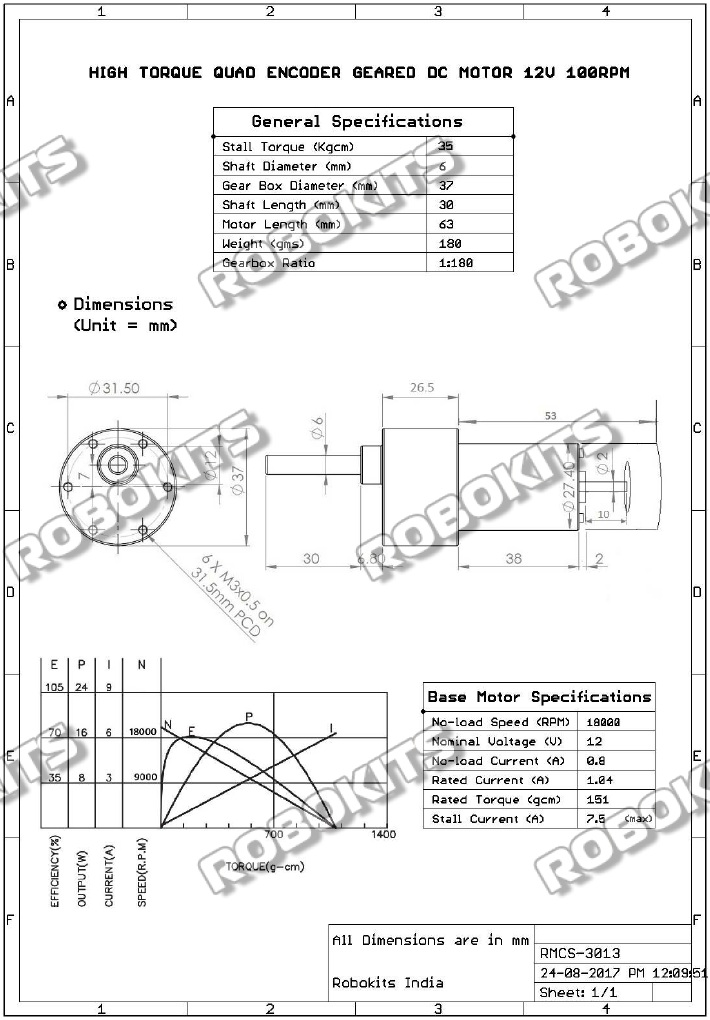
\includegraphics[scale=.35]{Motor_Datasheet.jpg}
	\end{center}
	\begin{center}
		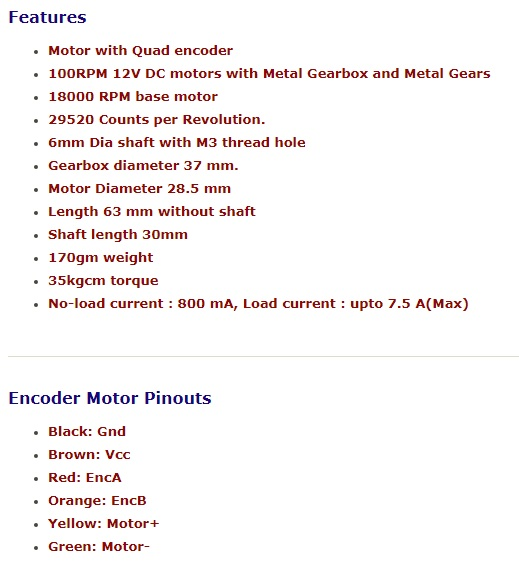
\includegraphics[scale=.55]{encoder_motor.jpg}
	\end{center}
  \item Motor Drivers pinouts:
	\begin{center}
		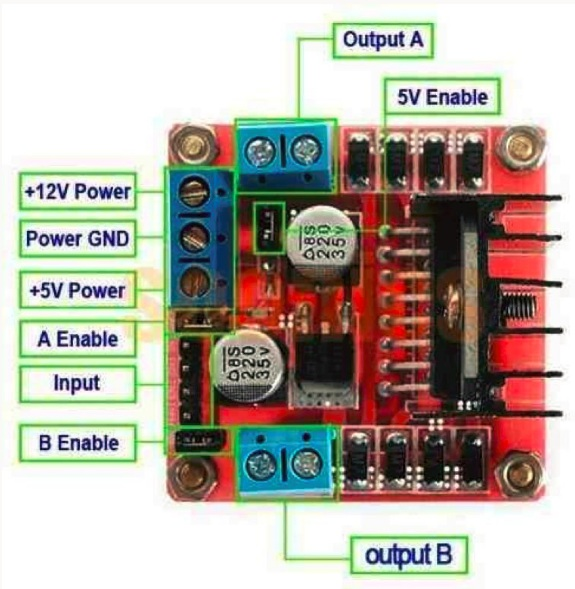
\includegraphics[scale=.55]{motor_driver_pinouts.jpg}
	\end{center}
  \item Raspberry Pi:
	\begin{center}
		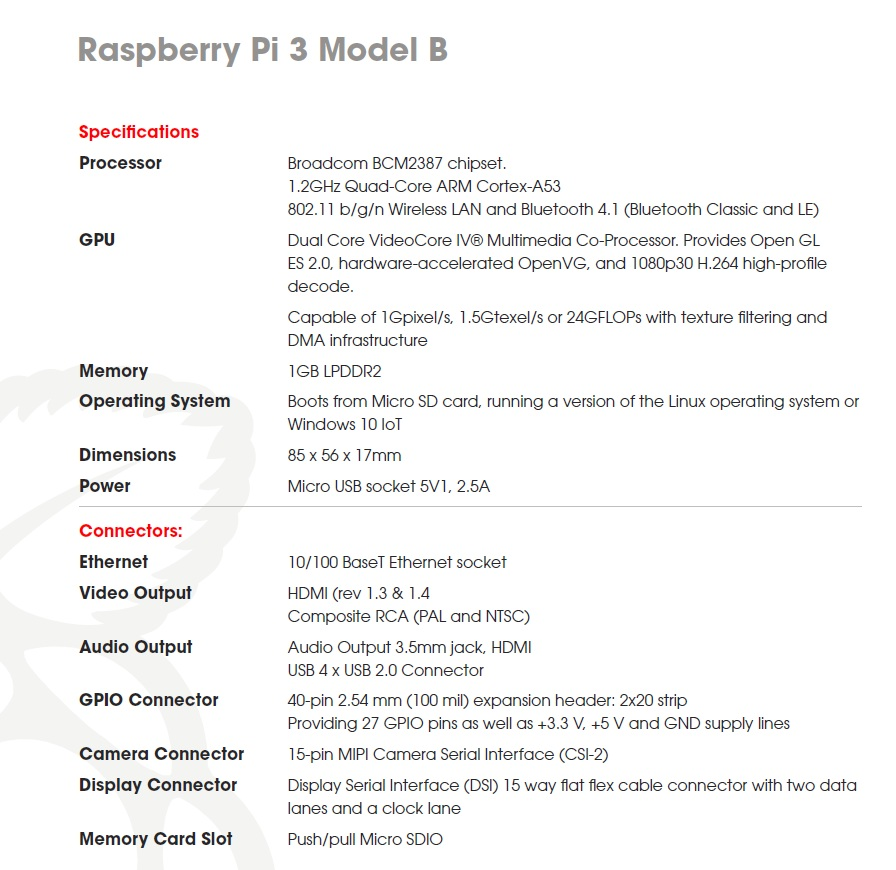
\includegraphics[scale=.4]{Raspberry_Pi_datasheet.jpg}
	\end{center}
  \item Arduino Mega board
	\begin{center}
		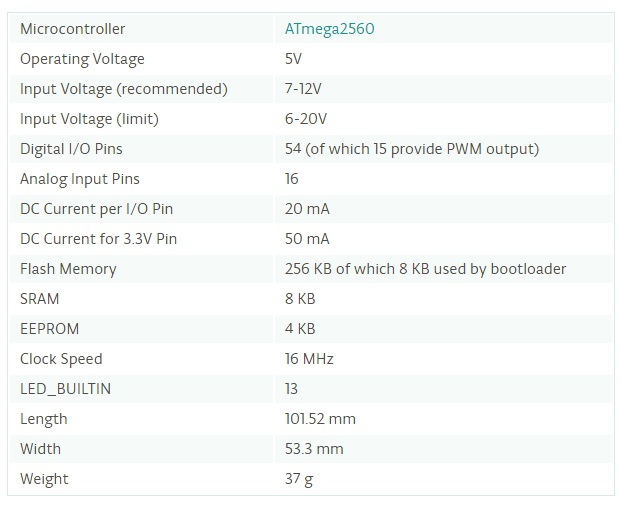
\includegraphics[scale=.6]{Arduinoboard_datasheet.jpg}
	\end{center}
\end{itemize}



\section{Software and libraries used}
\begin{itemize}
  \item From mechanical side we have used:
	\begin{itemize}
	\item Solid works software:
	\begin{center}
		
\includegraphics[scale=.2]{solidworks_home_page.jpg}
	\end{center}
		\begin{itemize}
		\item This software is a product of Dassault Systemes.
		\item This software is used for mechanical designing.
		\end{itemize}
	\item Ansys software:
	\begin{center}
		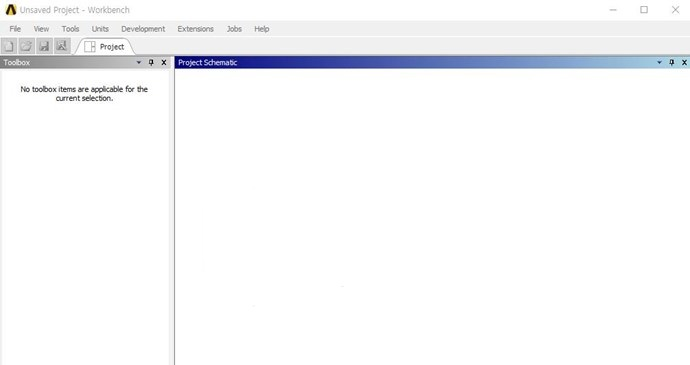
\includegraphics[scale=.5]{asys_home_page.jpg}
	\end{center}
		\begin{itemize}
		\item This software is a product of Ansys, Inc..
		\item This software is used for doing analysis which helps to find out the failure of the part at which particular load.
		\end{itemize}
	\end{itemize}
\end{itemize}
\begin{itemize}
    \item For image processing:
        \begin{itemize}
            \item OpenCV 3 
                \begin{itemize}
                    \item This library was made use of for handling all the image related processing.
                    \item To detect the corners of the trough and hence its location with respect to the frame.
                    \item To initialize the coordinate system with help of red marker denoting the origin of the whole system.
                \end{itemize}
                \begin{center}
                    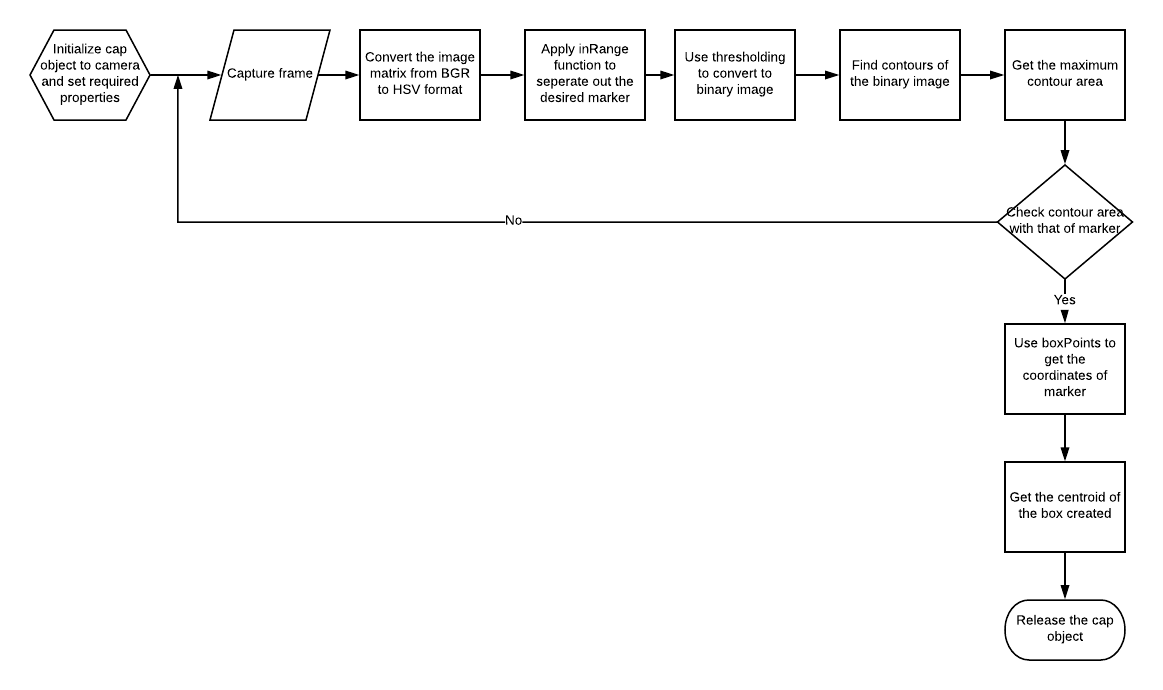
\includegraphics[scale=.5]{image_processing_1.png}
                \end{center}
        \end{itemize}
        
        \begin{itemize}
            \item tkinter library 
                \begin{itemize}
                    \item This library was used to create a windows application for user to interact with and fill in his or her requirements.  
                \end{itemize}
                \begin{center}
                    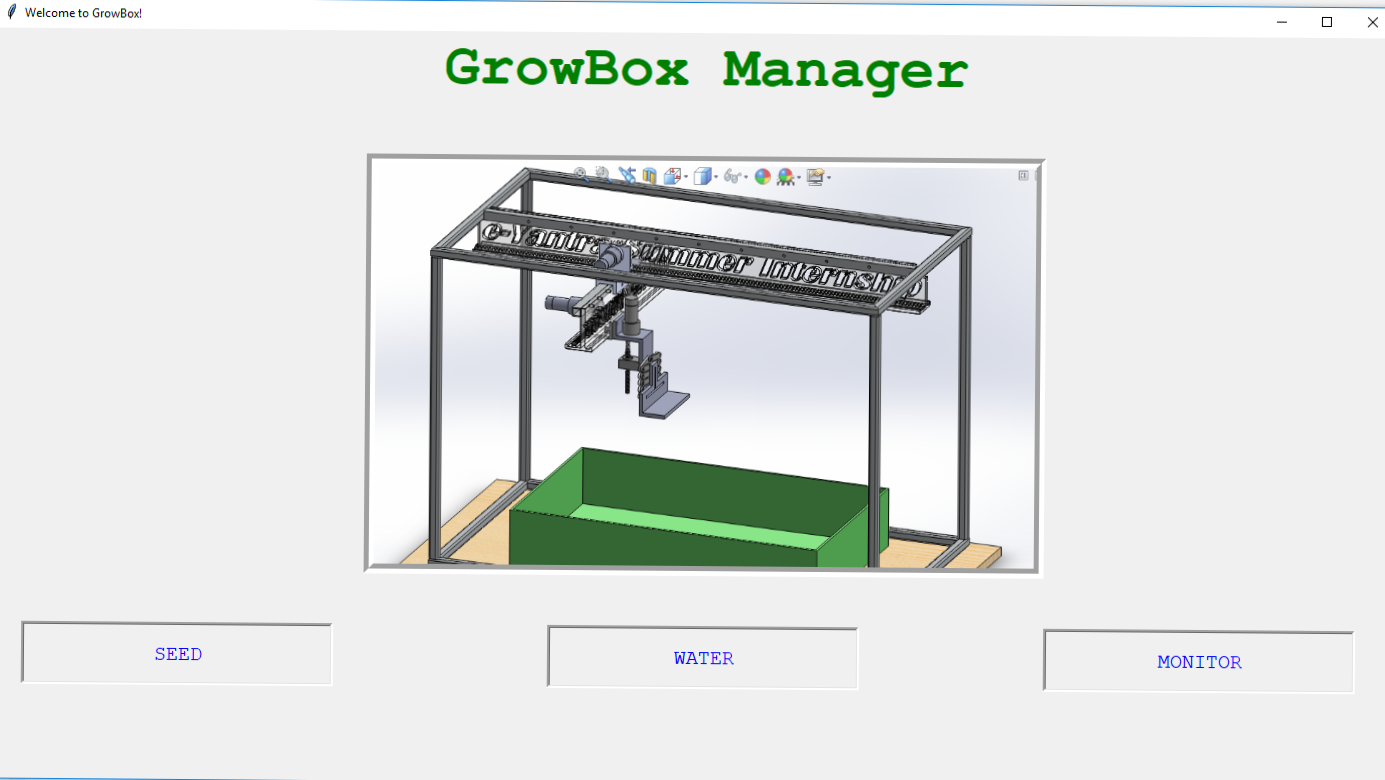
\includegraphics[scale=.3]{main_menu.png}
                \end{center}
                \begin{center}
                    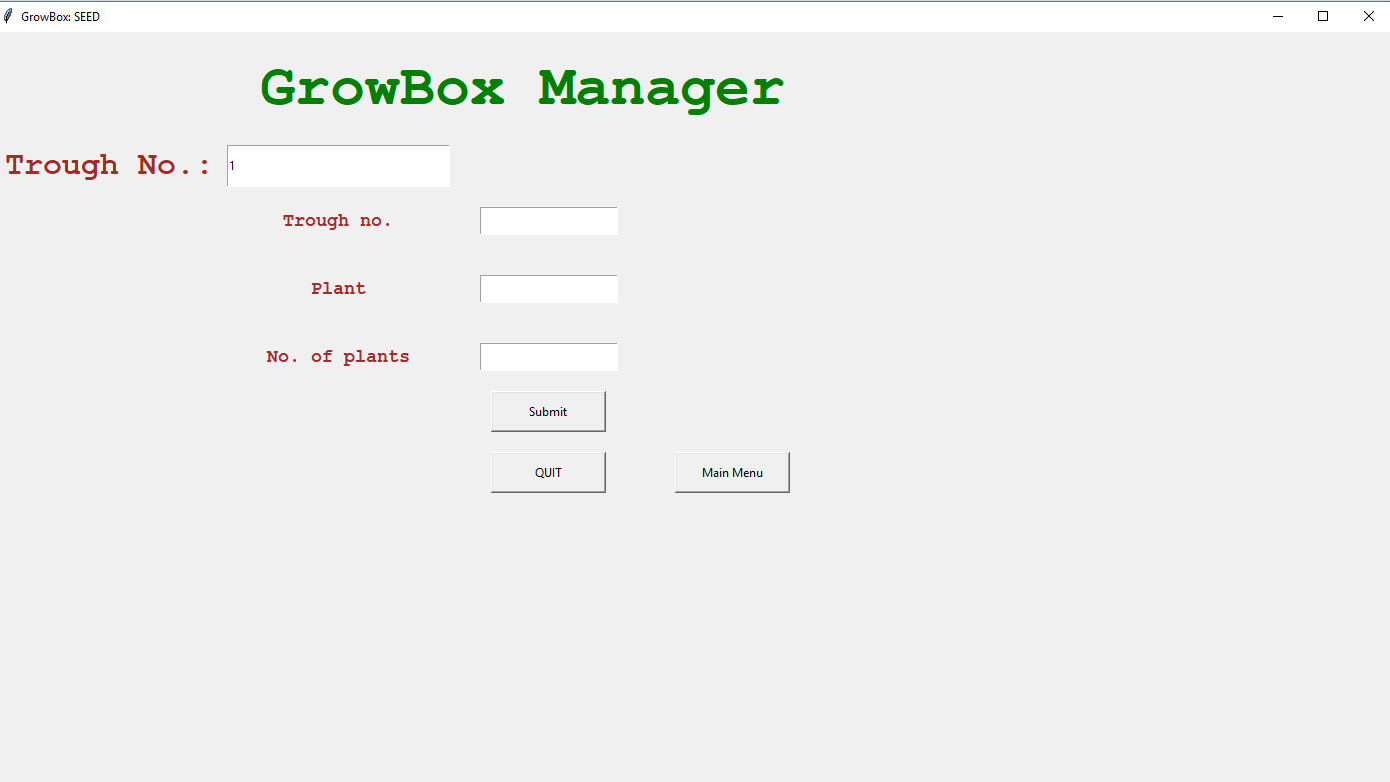
\includegraphics[scale=0.3]{seed_without_data.png}
                    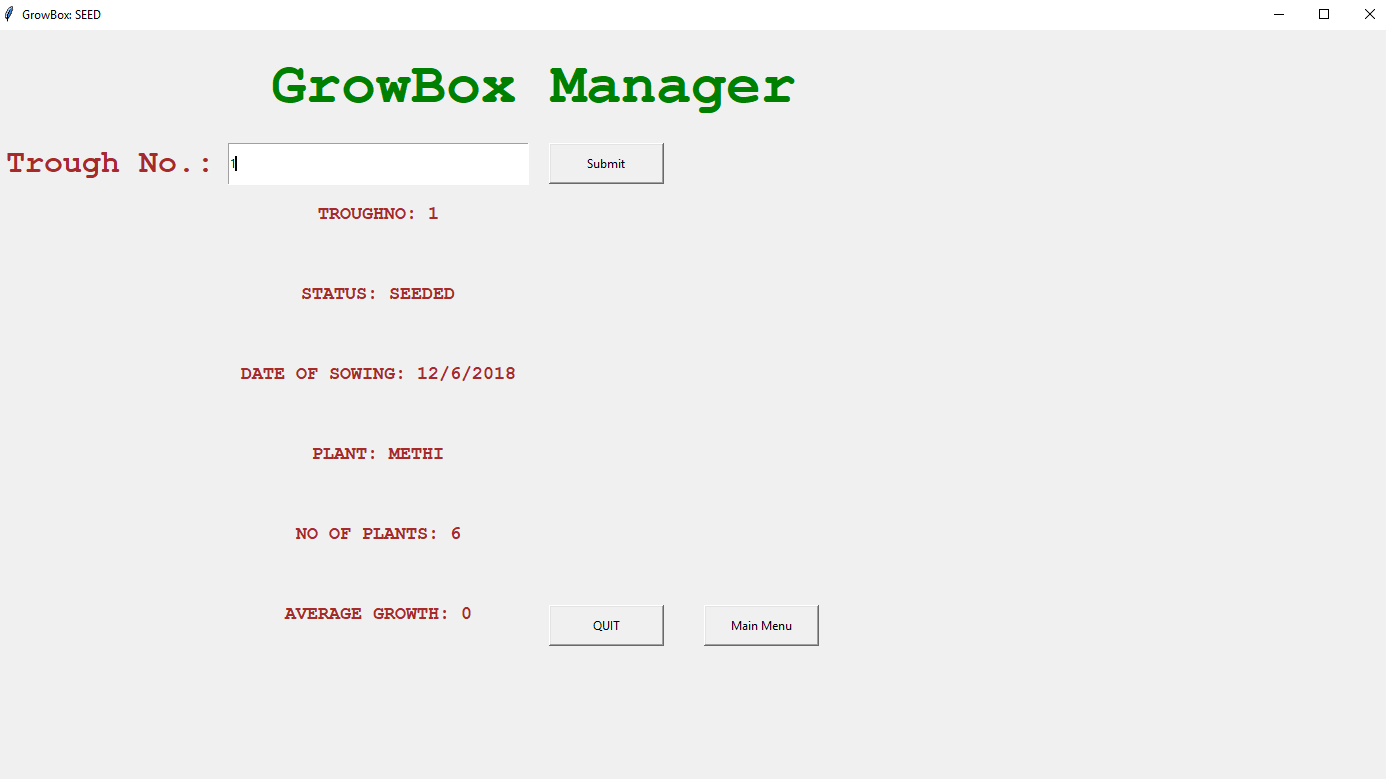
\includegraphics[scale=0.3]{seed_with_data.png}
                \end{center}
            \item GUI file execution flow 
            \begin{center}
                    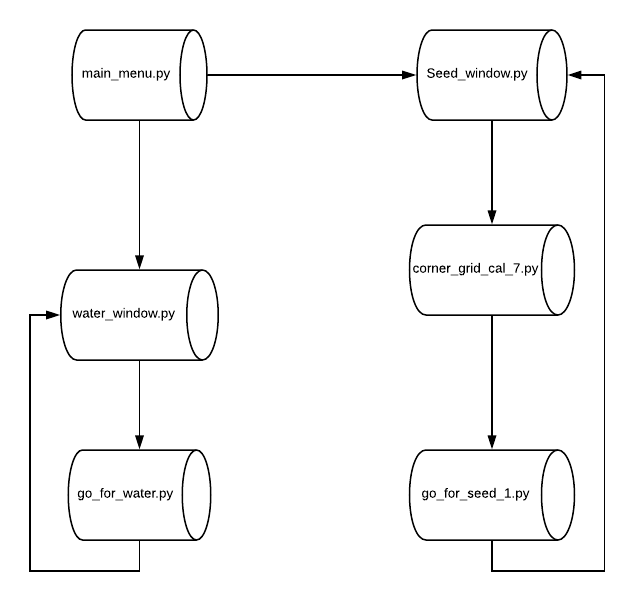
\includegraphics[scale=.5]{gui_flow.png}
                \end{center}
        \end{itemize}
\end{itemize}

\section{Assembly of hardware}

Below link guide about the whole mechanical assembly of the CNC.
\href{https://youtu.be/BbIcM0a_Fmc}{CNC for Growbox (assembly)} 
\subsection*{Circuit Diagram}
	\begin{center}
		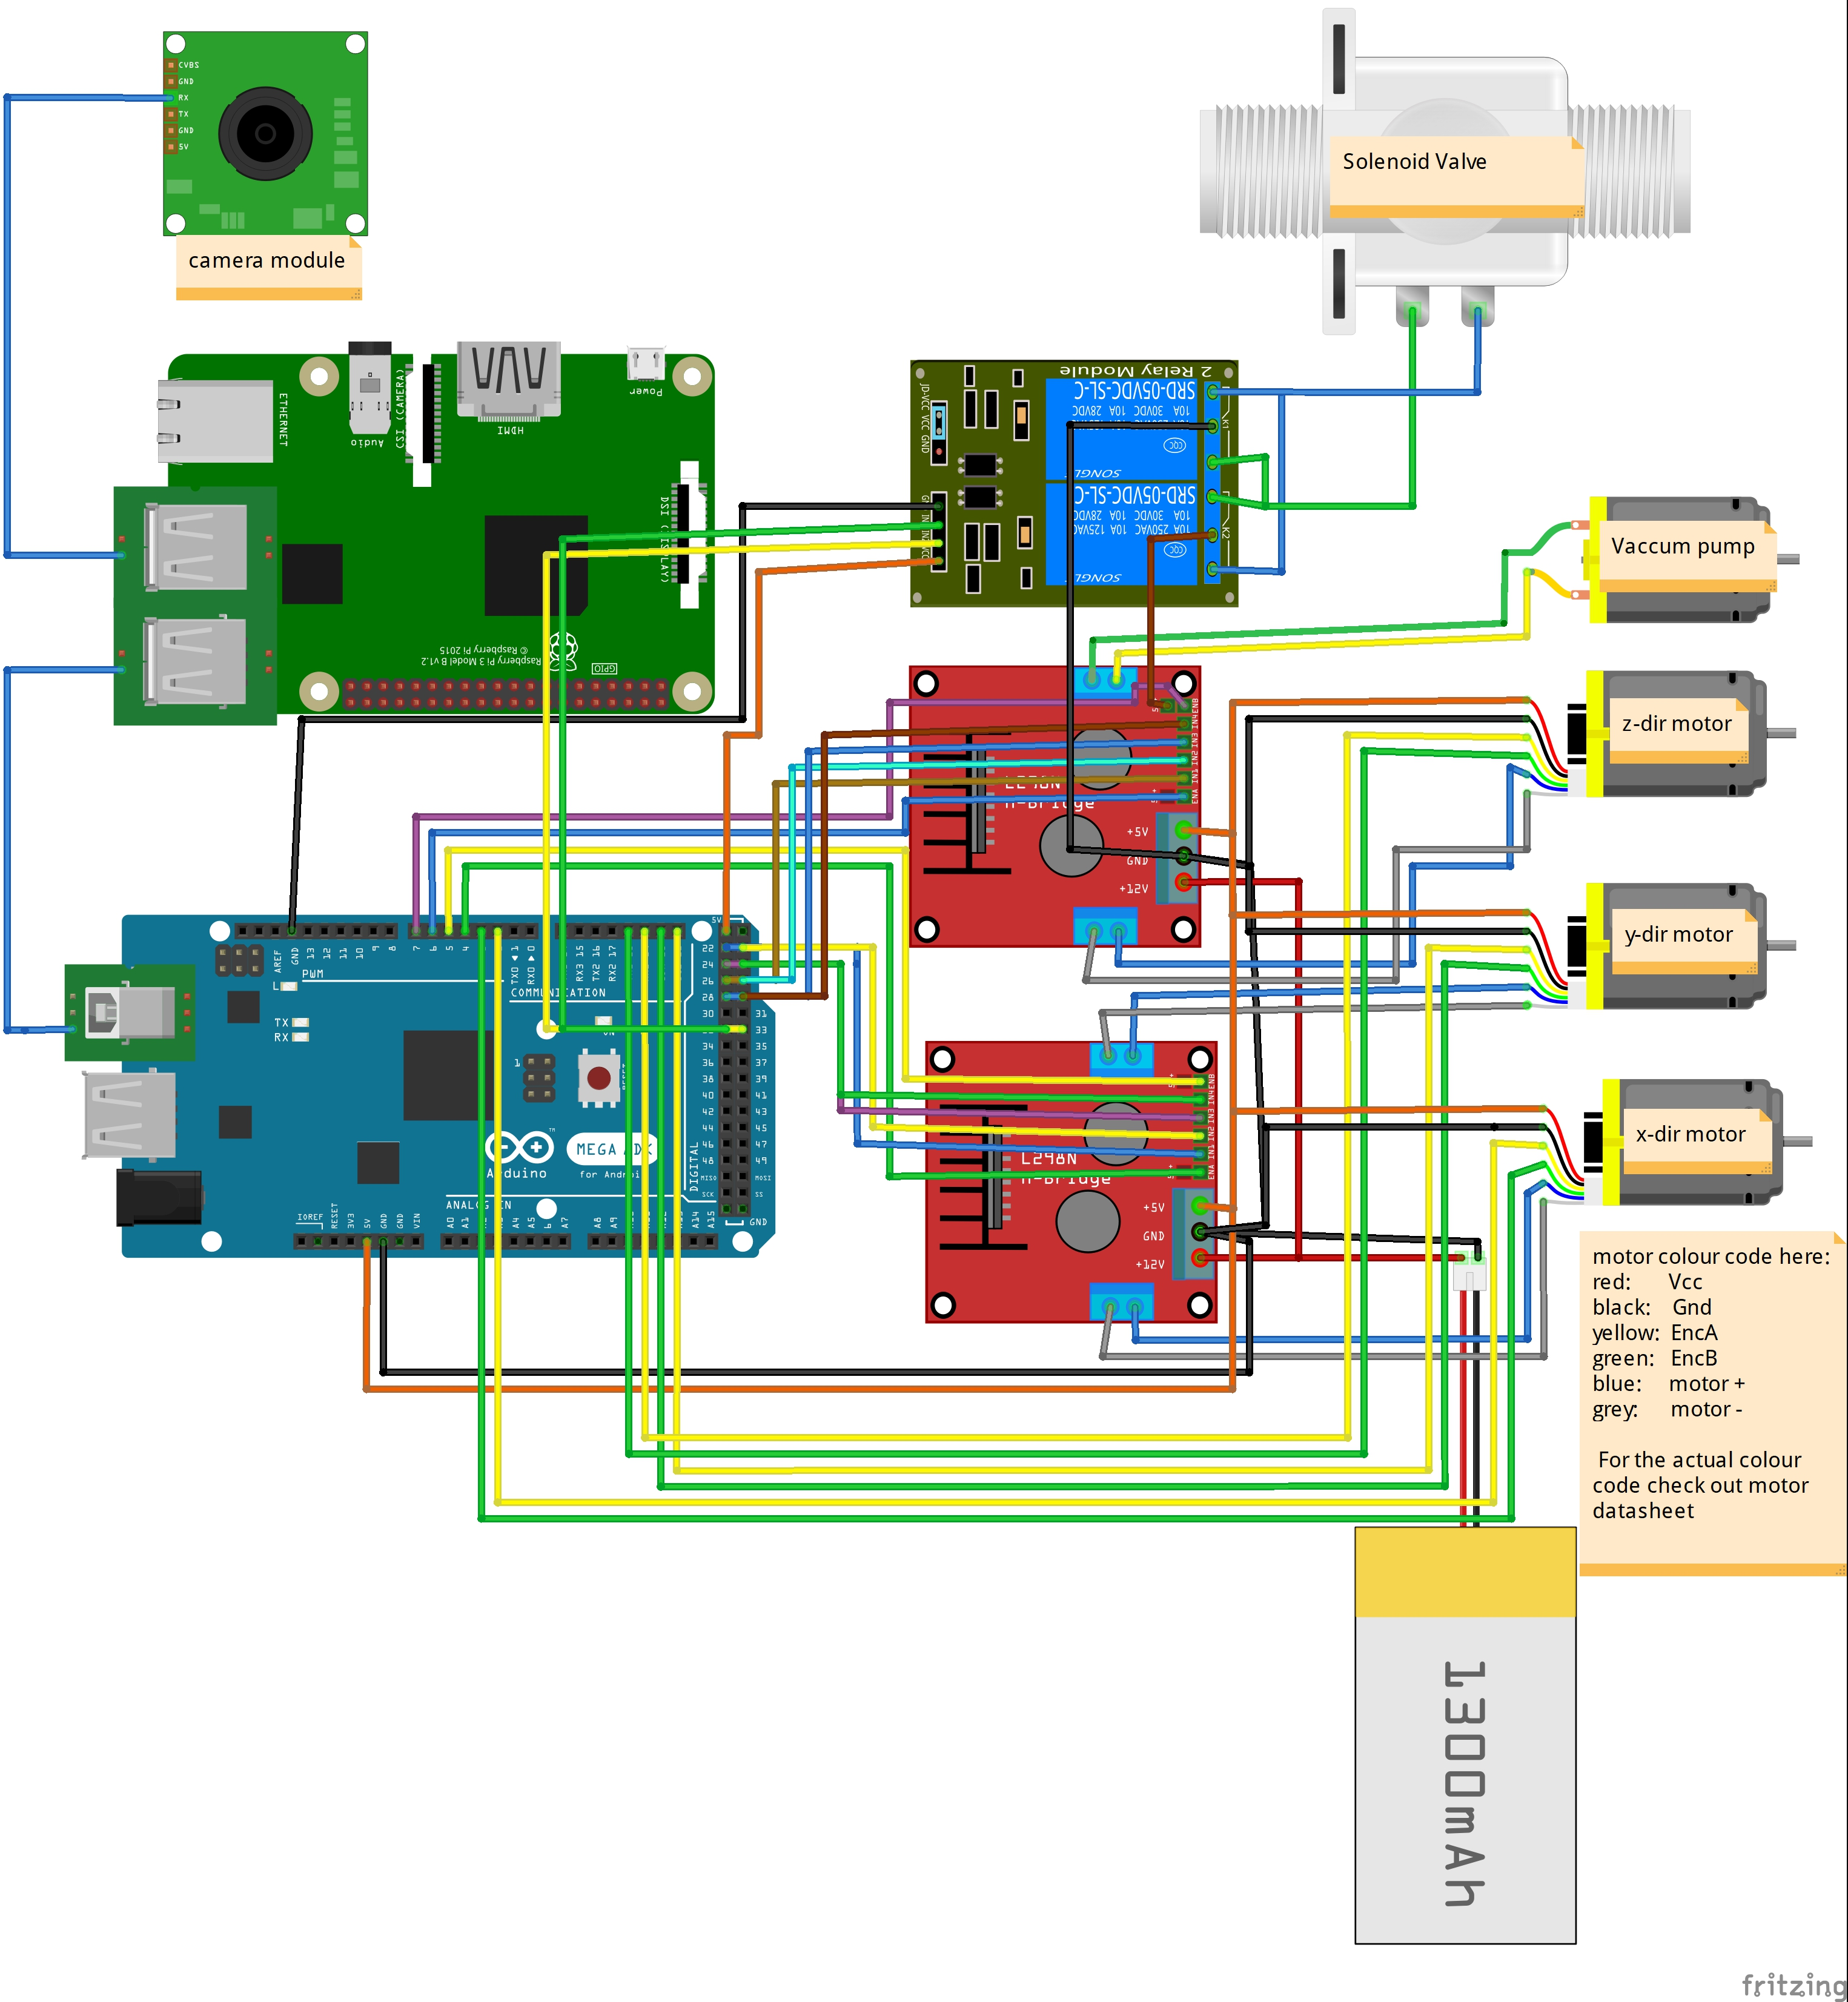
\includegraphics[scale=.3]{circuit_diagram_bb.jpg}
	\end{center}

\section{Software and Code}
\href{https://github.com/eYSIP-2018/CNC-for-GrowBox.git}{Github link} for the repository of code
\subsection*{Corner Detection and Coordinate initialization}
\begin{center}
    \item The flow chart of the program is as follows:
    \begin{center}
        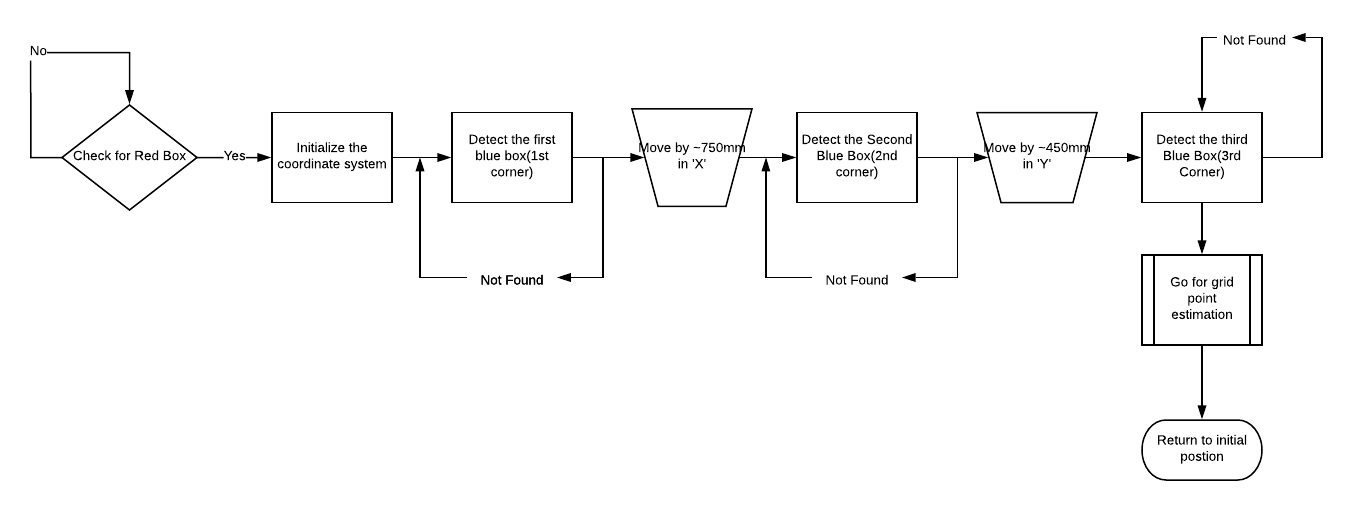
\includegraphics[scale=0.5]{Grid_coord_ini.png}
        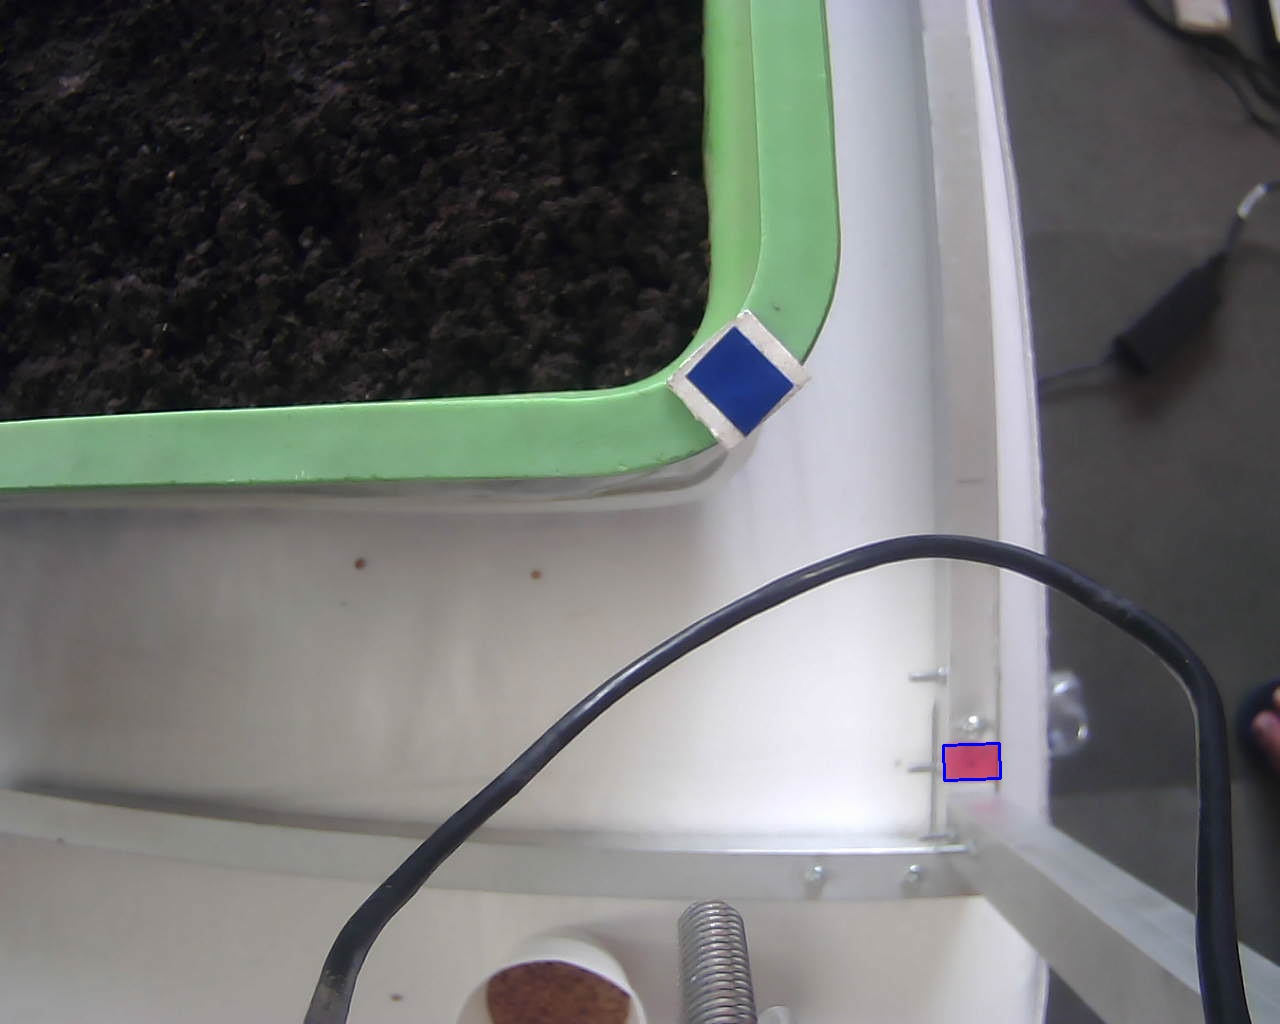
\includegraphics[scale=0.3]{img00.jpg}
        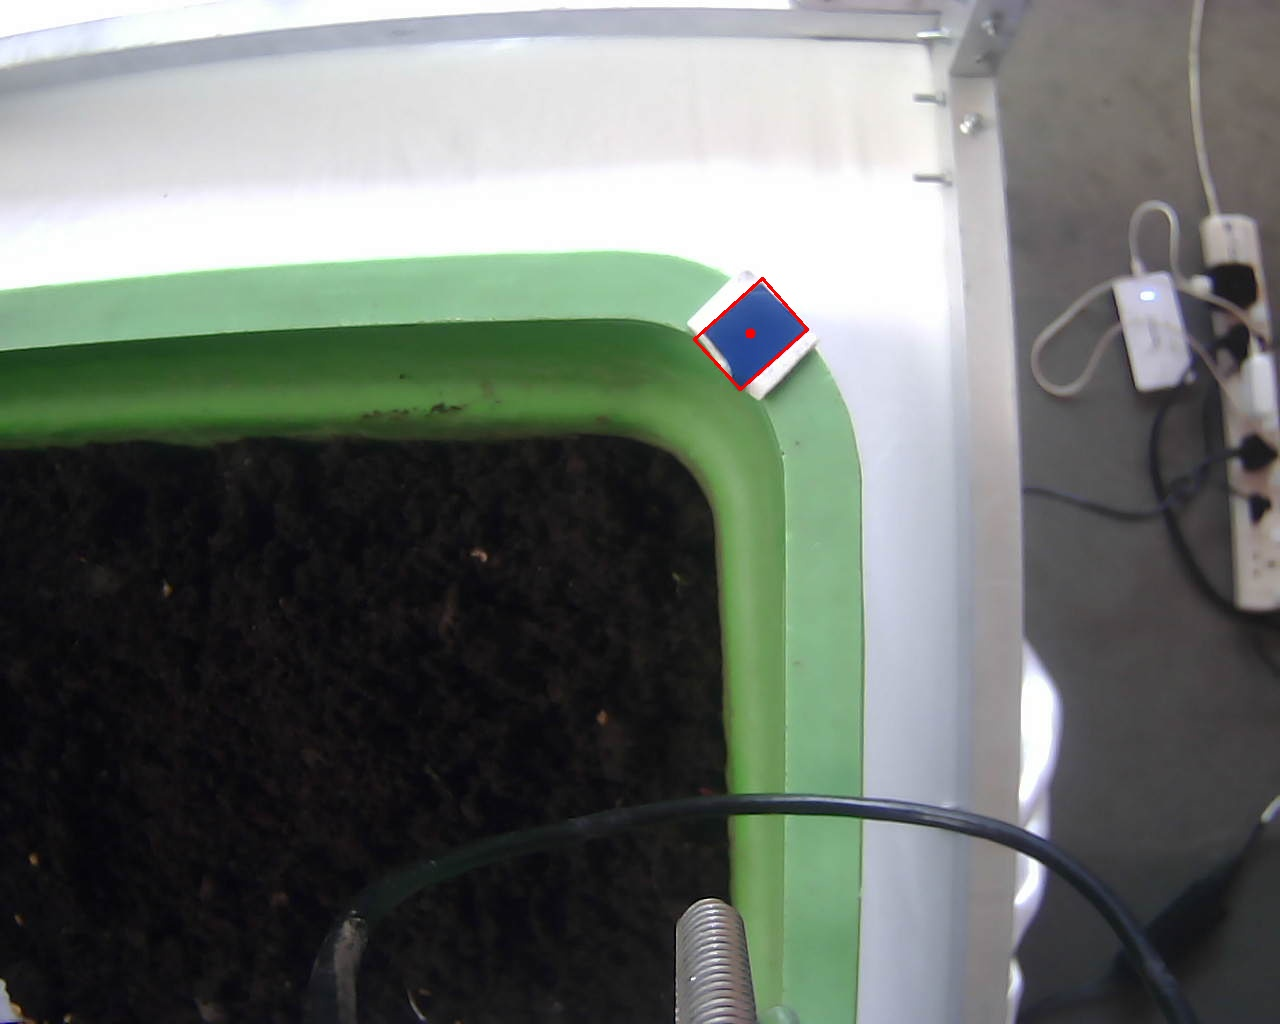
\includegraphics[scale=0.3]{img02.jpg}
    \end{center}
\end{center}
\subsection*{Seeding}
\begin{center}
    \item The flow chart of the program is as follows:
    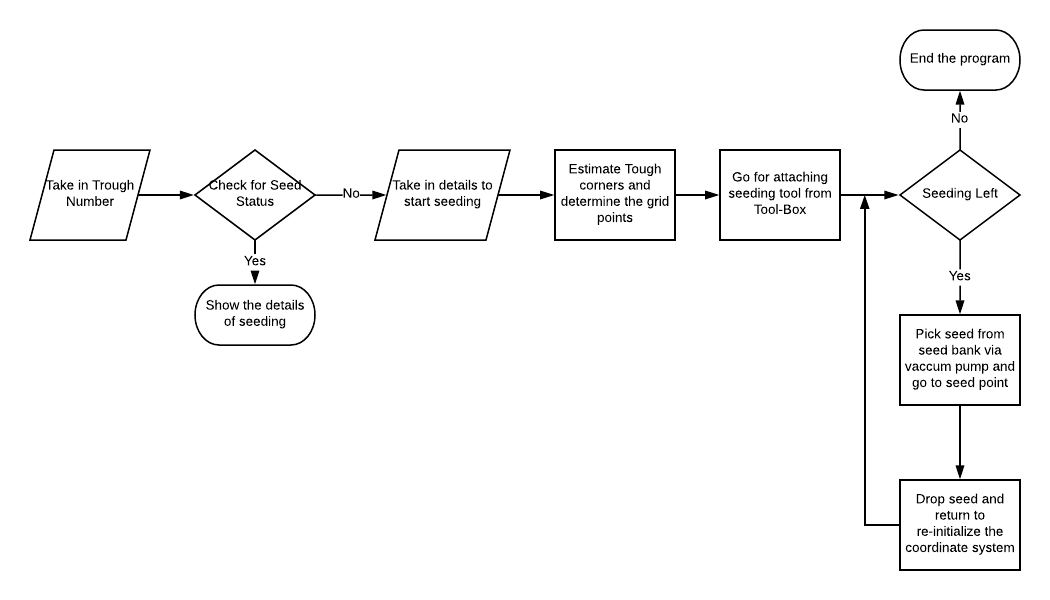
\includegraphics[scale=0.5]{seeding_for_document.png}    
\end{center}
\subsection*{Watering}
\begin{center}
    \item The flow chart of the program is as follows:
    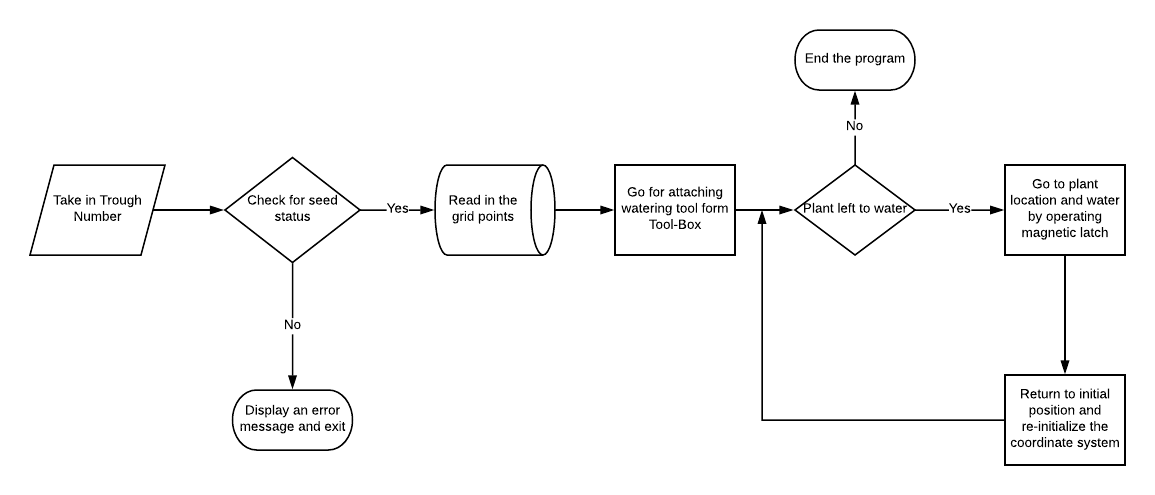
\includegraphics[scale=0.5]{water_for_document.png}    
\end{center}
\section{Use and Demo}
	\begin{center}
		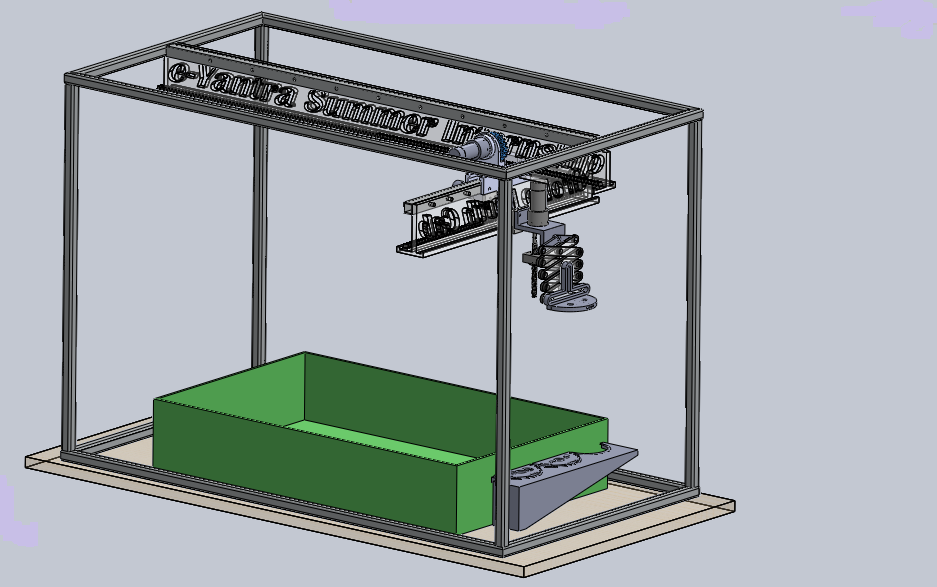
\includegraphics[scale=.6]{design.png}
	\end{center}
	\begin{center}
		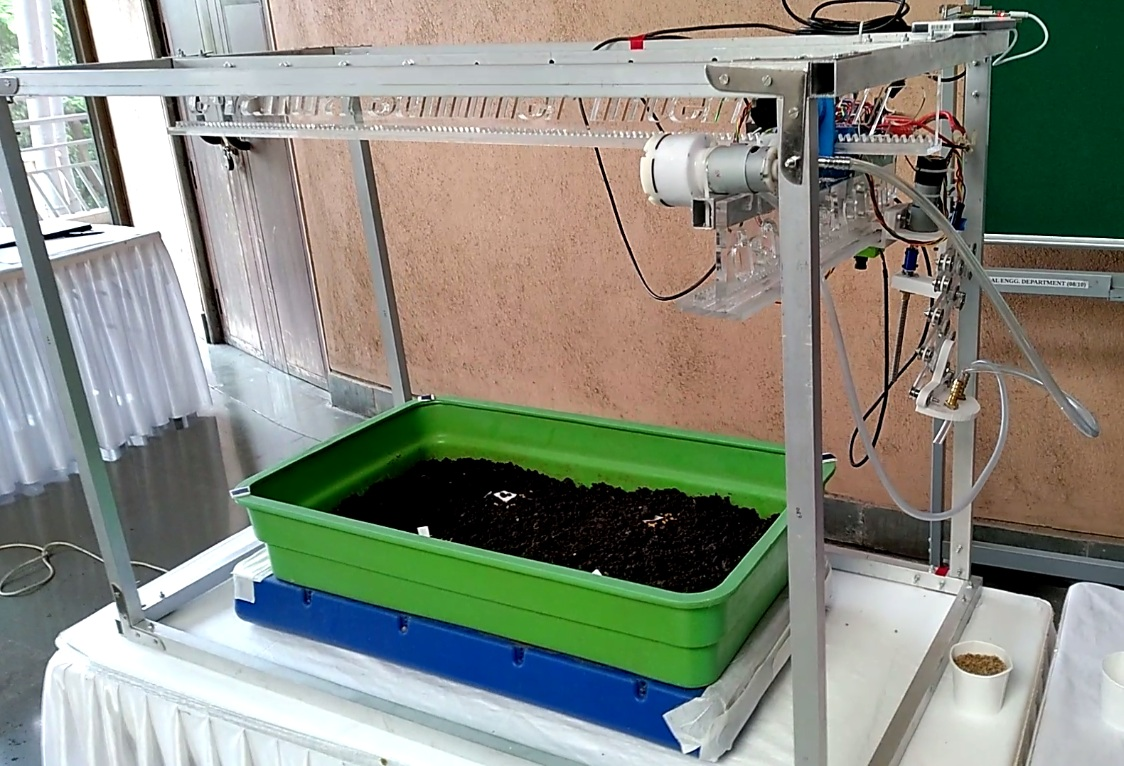
\includegraphics[scale=.5]{growbox_image.jpg}
	\end{center}

\href{https://youtu.be/hDnJ0aEMh-A}{CNC for Growbox (working)} of demonstration video 

\section{Features}
\begin{itemize}
    \item It has the ability to serve multiple groboxes placed in a row.
    \item It can seed as well as water them automatically.
    \item Light in weight and thus easy to transfer it from one place to another.
    \item You can place trough at any place and orientation inside the frame.
    \item We can input the number of plants to be seeded through the GUI we created.
\end{itemize}

\section{Future Work}
As there is always a room for improvement; there are some of them in our project too:
\begin{itemize}
    \item Firstly, we need to make this whole mechanism as compact as possible so less room is required for its placement.
    \item We needed to give either two supports instead of one at the top or figure out some other mechanism which can give rigid support to the whole CNC without vibration.
    \item We can add detachable tools instead of universal one for different actions such as watering, seeding, etc.
    \item Position of all the tools and seed carrying container should be fixed so tool head will be able to collect them automatically as per requirement.
    \item Instead of picking single seed in one go we pick whole bunch of seeds and place it individually at every different place of the grid point.
    \item It can also be designed to shift grow boxes in rows as well as columns thus covering growboxes in large area.
    \item It should also be able to monitor the plant growth and identify the seeds and make the grid points such that it should satisfy the need of minimum space requirement for that particular plant.
    \item There should be an user friendly android app which can help to operate the CNC by sitting any corner of the world.
    \item This system should be able to pick seeds in its proper orientation and drop at the depth required by that kind of seeds for its proper growth.
    \item Plant health monitoring can be achieved with the help of machine learning and image processing.
\end{itemize}

\section{Bug report and Challenges}
Challenges faced in Hardware design:
    \begin{itemize}
        \item Due to the single L-clamp used for fitting of the frame, causes vibration of the whole structure.
        \item As while designing we gave single support to the CNC mechanisms from the top and that too, was very bulky after manufacturing it, whole mechanism was vibrating.
        \item Also, we didn't give any support to the lead-screw for the z-axis motion(vertical) thus lead-screw was bending alot.
        \item We also designed watering and seed picking tools but were not able to avoid the leakages.
        \item We didn't attach any kind of stoppages on the rails which are used for x and y-axis motion due to which many of the times during malfunctioning error whole mechanism came out of the rail.
    \end{itemize}
Challenges faced in Electronics
    \begin{itemize}
        \item We used pin to pin connectors and motor relimates which created problem of loose connections.
        \item We forgot to use input pull-ups for encoder pins that wasted our time.
        \item Solenoid has to be run through separate driver  with high current power supply instead of using relays with 5V supply from motor driver.
    \end{itemize}
Challenges faced in Image Processing 
    \begin{itemize}
        \item Initially we had planned to use pi camera which had issues like the soldering was not robust enough leading to no collection of sensor data several times or in some cases, not even capturing a frame. 
        \item The grid point estimation had to be dynamic, i.e., should not depend on orientation and placement of the trough with respect to the frame.
        \item The camera would take either a lot of time to adjust to ambient light or it would just capture photos dull enough to fail the image processing to give desired result. An experimental exposure value had to be set to make the whole process robust. 
        \item Trough corner detection was first decided to be dependent on the actual border, whose contour would be extracted and an approximate polygon would be found to extract a point for future grid calculation. However, this approach was giving a lot of uncertainty to whole process, therefore blue markers were used to get corner coordinates. This helped us to estimate the grid coordinates very accurately. 
    \end{itemize}

\begin{thebibliography}{li}
\bibitem{wavelan97}
Ad Kamerman and Leo Monteban,
{\em WaveLAN-II: A High-Performance Wireless LAN for the Unlicensed band},
1997.

\end{thebibliography}


\end{document}

